\documentclass[1p]{elsarticle_modified}
%\bibliographystyle{elsarticle-num}

%\usepackage[colorlinks]{hyperref}
%\usepackage{abbrmath_seonhwa} %\Abb, \Ascr, \Acal ,\Abf, \Afrak
\usepackage{amsfonts}
\usepackage{amssymb}
\usepackage{amsmath}
\usepackage{amsthm}
\usepackage{scalefnt}
\usepackage{amsbsy}
\usepackage{kotex}
\usepackage{caption}
\usepackage{subfig}
\usepackage{color}
\usepackage{graphicx}
\usepackage{xcolor} %% white, black, red, green, blue, cyan, magenta, yellow
\usepackage{float}
\usepackage{setspace}
\usepackage{hyperref}

\usepackage{tikz}
\usetikzlibrary{arrows}

\usepackage{multirow}
\usepackage{array} % fixed length table
\usepackage{hhline}

%%%%%%%%%%%%%%%%%%%%%
\makeatletter
\renewcommand*\env@matrix[1][\arraystretch]{%
	\edef\arraystretch{#1}%
	\hskip -\arraycolsep
	\let\@ifnextchar\new@ifnextchar
	\array{*\c@MaxMatrixCols c}}
\makeatother %https://tex.stackexchange.com/questions/14071/how-can-i-increase-the-line-spacing-in-a-matrix
%%%%%%%%%%%%%%%

\usepackage[normalem]{ulem}

\newcommand{\msout}[1]{\ifmmode\text{\sout{\ensuremath{#1}}}\else\sout{#1}\fi}
%SOURCE: \msout is \stkout macro in https://tex.stackexchange.com/questions/20609/strikeout-in-math-mode

\newcommand{\cancel}[1]{
	\ifmmode
	{\color{red}\msout{#1}}
	\else
	{\color{red}\sout{#1}}
	\fi
}

\newcommand{\add}[1]{
	{\color{blue}\uwave{#1}}
}

\newcommand{\replace}[2]{
	\ifmmode
	{\color{red}\msout{#1}}{\color{blue}\uwave{#2}}
	\else
	{\color{red}\sout{#1}}{\color{blue}\uwave{#2}}
	\fi
}

\newcommand{\Sol}{\mathcal{S}} %segment
\newcommand{\D}{D} %diagram
\newcommand{\A}{\mathcal{A}} %arc


%%%%%%%%%%%%%%%%%%%%%%%%%%%%%5 test

\def\sl{\operatorname{\textup{SL}}(2,\Cbb)}
\def\psl{\operatorname{\textup{PSL}}(2,\Cbb)}
\def\quan{\mkern 1mu \triangleright \mkern 1mu}

\theoremstyle{definition}
\newtheorem{thm}{Theorem}[section]
\newtheorem{prop}[thm]{Proposition}
\newtheorem{lem}[thm]{Lemma}
\newtheorem{ques}[thm]{Question}
\newtheorem{cor}[thm]{Corollary}
\newtheorem{defn}[thm]{Definition}
\newtheorem{exam}[thm]{Example}
\newtheorem{rmk}[thm]{Remark}
\newtheorem{alg}[thm]{Algorithm}

\newcommand{\I}{\sqrt{-1}}
\begin{document}

%\begin{frontmatter}
%
%\title{Boundary parabolic representations of knots up to 8 crossings}
%
%%% Group authors per affiliation:
%\author{Yunhi Cho} 
%\address{Department of Mathematics, University of Seoul, Seoul, Korea}
%\ead{yhcho@uos.ac.kr}
%
%
%\author{Seonhwa Kim} %\fnref{s_kim}}
%\address{Center for Geometry and Physics, Institute for Basic Science, Pohang, 37673, Korea}
%\ead{ryeona17@ibs.re.kr}
%
%\author{Hyuk Kim}
%\address{Department of Mathematical Sciences, Seoul National University, Seoul 08826, Korea}
%\ead{hyukkim@snu.ac.kr}
%
%\author{Seokbeom Yoon}
%\address{Department of Mathematical Sciences, Seoul National University, Seoul, 08826,  Korea}
%\ead{sbyoon15@snu.ac.kr}
%
%\begin{abstract}
%We find all boundary parabolic representation of knots up to 8 crossings.
%
%\end{abstract}
%\begin{keyword}
%    \MSC[2010] 57M25 
%\end{keyword}
%
%\end{frontmatter}

%\linenumbers
%\tableofcontents
%
\newcommand\colored[1]{\textcolor{white}{\rule[-0.35ex]{0.8em}{1.4ex}}\kern-0.8em\color{red} #1}%
%\newcommand\colored[1]{\textcolor{white}{ #1}\kern-2.17ex	\textcolor{white}{ #1}\kern-1.81ex	\textcolor{white}{ #1}\kern-2.15ex\color{red}#1	}

{\Large $\underline{12n_{0587}~(K12n_{0587})}$}

\setlength{\tabcolsep}{10pt}
\renewcommand{\arraystretch}{1.6}
\vspace{1cm}\begin{tabular}{m{100pt}>{\centering\arraybackslash}m{274pt}}
\multirow{5}{120pt}{
	\centering
	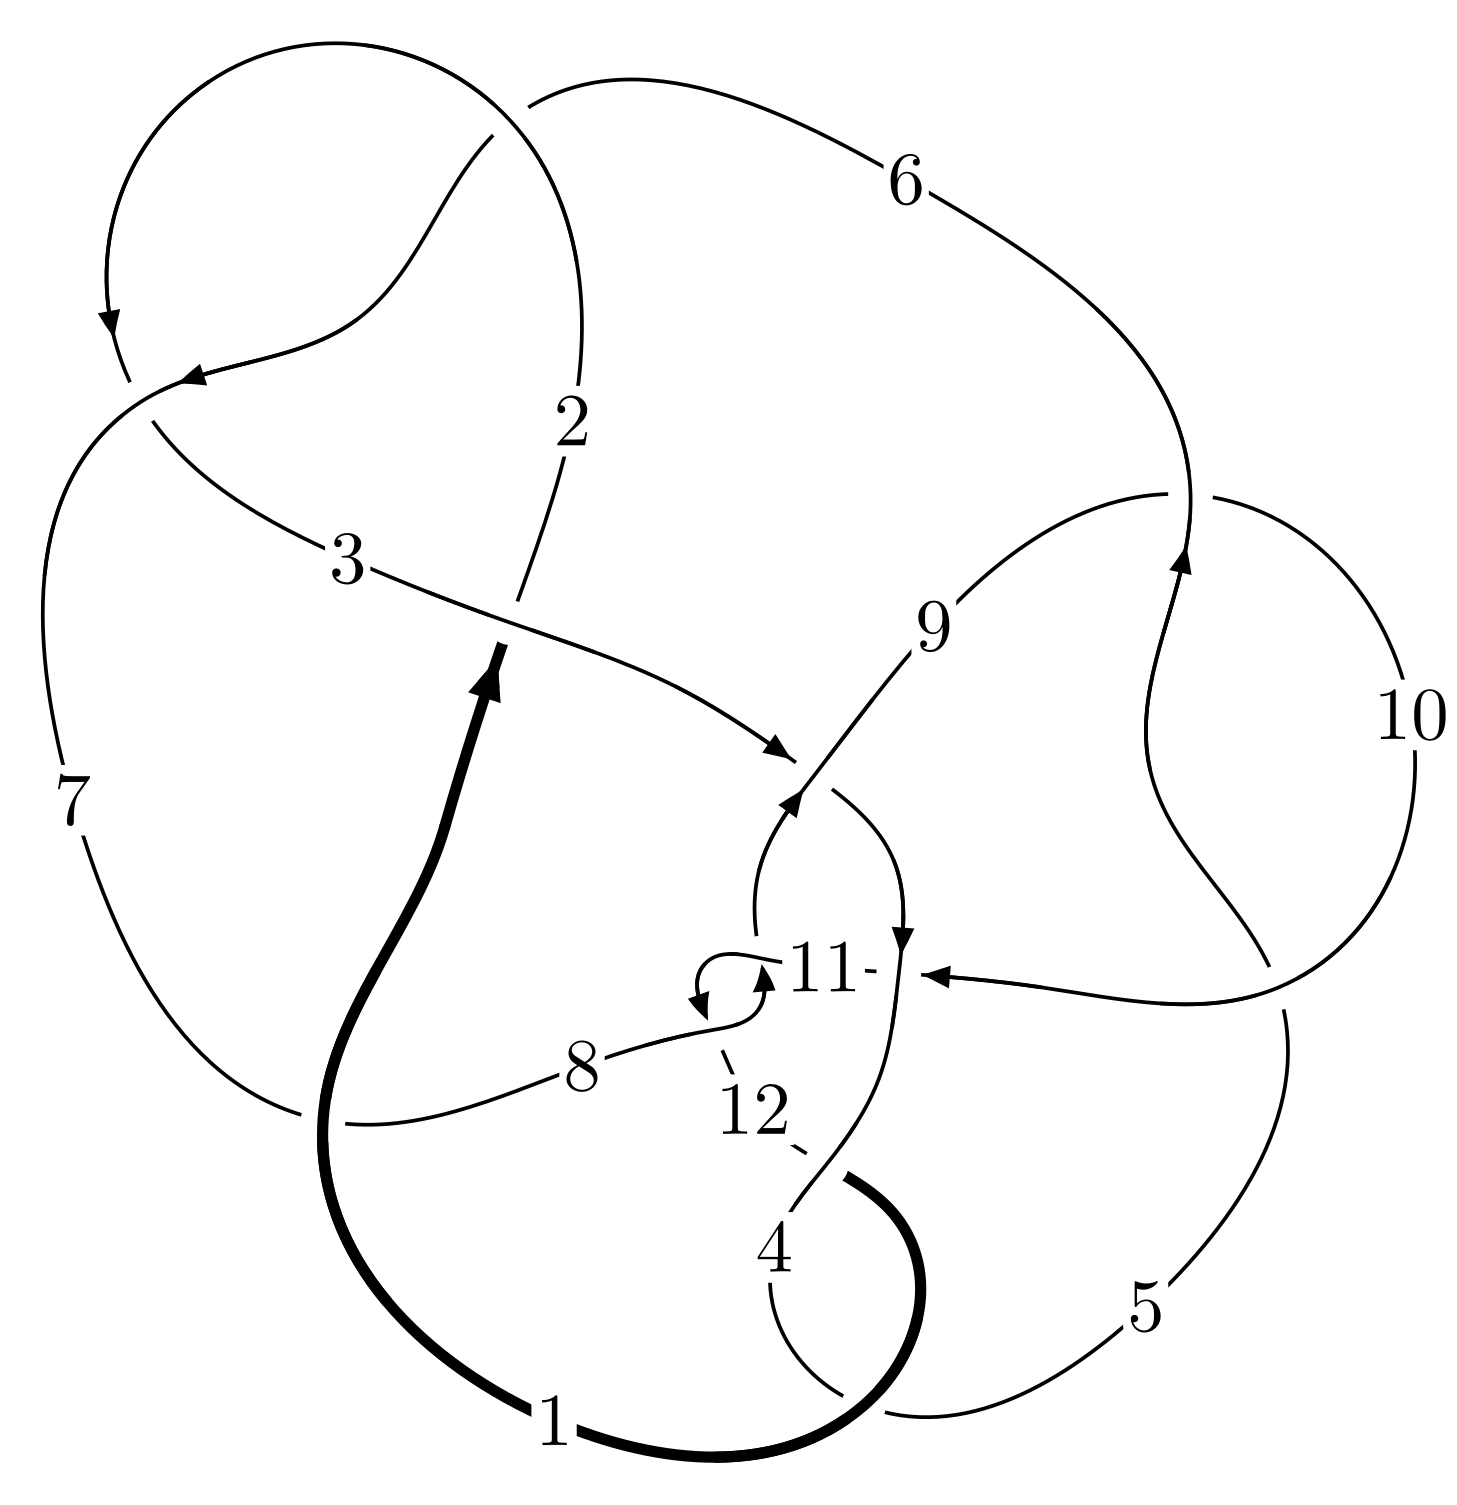
\includegraphics[width=112pt]{../../../GIT/diagram.site/Diagrams/png/2676_12n_0587.png}\\
\ \ \ A knot diagram\footnotemark}&
\allowdisplaybreaks
\textbf{Linearized knot diagam} \\
\cline{2-2}
 &
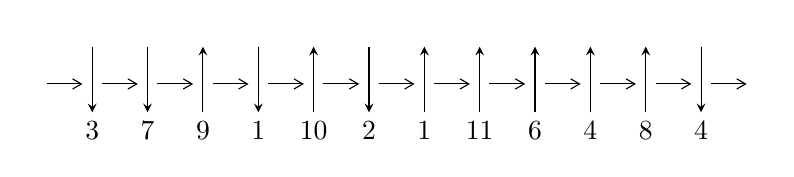
\begin{tikzpicture}[x=20pt, y=17pt]
	% nodes
	\node (C0) at (0, 0) {};
	\node (C1) at (1, 0) {};
	\node (C1U) at (1, +1) {};
	\node (C1D) at (1, -1) {3};

	\node (C2) at (2, 0) {};
	\node (C2U) at (2, +1) {};
	\node (C2D) at (2, -1) {7};

	\node (C3) at (3, 0) {};
	\node (C3U) at (3, +1) {};
	\node (C3D) at (3, -1) {9};

	\node (C4) at (4, 0) {};
	\node (C4U) at (4, +1) {};
	\node (C4D) at (4, -1) {1};

	\node (C5) at (5, 0) {};
	\node (C5U) at (5, +1) {};
	\node (C5D) at (5, -1) {10};

	\node (C6) at (6, 0) {};
	\node (C6U) at (6, +1) {};
	\node (C6D) at (6, -1) {2};

	\node (C7) at (7, 0) {};
	\node (C7U) at (7, +1) {};
	\node (C7D) at (7, -1) {1};

	\node (C8) at (8, 0) {};
	\node (C8U) at (8, +1) {};
	\node (C8D) at (8, -1) {11};

	\node (C9) at (9, 0) {};
	\node (C9U) at (9, +1) {};
	\node (C9D) at (9, -1) {6};

	\node (C10) at (10, 0) {};
	\node (C10U) at (10, +1) {};
	\node (C10D) at (10, -1) {4};

	\node (C11) at (11, 0) {};
	\node (C11U) at (11, +1) {};
	\node (C11D) at (11, -1) {8};

	\node (C12) at (12, 0) {};
	\node (C12U) at (12, +1) {};
	\node (C12D) at (12, -1) {4};
	\node (C13) at (13, 0) {};

	% arrows
	\draw[->,>={angle 60}]
	(C0) edge (C1) (C1) edge (C2) (C2) edge (C3) (C3) edge (C4) (C4) edge (C5) (C5) edge (C6) (C6) edge (C7) (C7) edge (C8) (C8) edge (C9) (C9) edge (C10) (C10) edge (C11) (C11) edge (C12) (C12) edge (C13) ;	\draw[->,>=stealth]
	(C1U) edge (C1D) (C2U) edge (C2D) (C3D) edge (C3U) (C4U) edge (C4D) (C5D) edge (C5U) (C6U) edge (C6D) (C7D) edge (C7U) (C8D) edge (C8U) (C9D) edge (C9U) (C10D) edge (C10U) (C11D) edge (C11U) (C12U) edge (C12D) ;
	\end{tikzpicture} \\
\hhline{~~} \\& 
\textbf{Solving Sequence} \\ \cline{2-2} 
 &
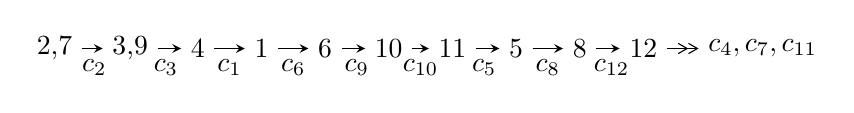
\begin{tikzpicture}[x=23pt, y=7pt]
	% node
	\node (A0) at (-1/8, 0) {2,7};
	\node (A1) at (17/16, 0) {3,9};
	\node (A2) at (17/8, 0) {4};
	\node (A3) at (25/8, 0) {1};
	\node (A4) at (33/8, 0) {6};
	\node (A5) at (41/8, 0) {10};
	\node (A6) at (49/8, 0) {11};
	\node (A7) at (57/8, 0) {5};
	\node (A8) at (65/8, 0) {8};
	\node (A9) at (73/8, 0) {12};
	\node (C1) at (1/2, -1) {$c_{2}$};
	\node (C2) at (13/8, -1) {$c_{3}$};
	\node (C3) at (21/8, -1) {$c_{1}$};
	\node (C4) at (29/8, -1) {$c_{6}$};
	\node (C5) at (37/8, -1) {$c_{9}$};
	\node (C6) at (45/8, -1) {$c_{10}$};
	\node (C7) at (53/8, -1) {$c_{5}$};
	\node (C8) at (61/8, -1) {$c_{8}$};
	\node (C9) at (69/8, -1) {$c_{12}$};
	\node (A10) at (11, 0) {$c_{4},c_{7},c_{11}$};

	% edge
	\draw[->,>=stealth]	
	(A0) edge (A1) (A1) edge (A2) (A2) edge (A3) (A3) edge (A4) (A4) edge (A5) (A5) edge (A6) (A6) edge (A7) (A7) edge (A8) (A8) edge (A9) ;
	\draw[->>,>={angle 60}]	
	(A9) edge (A10);
\end{tikzpicture} \\ 

\end{tabular} \\

\footnotetext{
The image of knot diagram is generated by the software ``\textbf{Draw programme}" developed by Andrew Bartholomew(\url{http://www.layer8.co.uk/maths/draw/index.htm\#Running-draw}), where we modified some parts for our purpose(\url{https://github.com/CATsTAILs/LinksPainter}).
}\phantom \\ \newline 
\centering \textbf{Ideals for irreducible components\footnotemark of $X_{\text{par}}$} 
 
\begin{align*}
I^u_{1}&=\langle 
-66 u^{31}-537 u^{30}+\cdots+4 b-972,\;-243 u^{31}-1923 u^{30}+\cdots+16 a-3048,\\
\phantom{I^u_{1}}&\phantom{= \langle  }u^{32}+9 u^{31}+\cdots+128 u+16\rangle \\
I^u_{2}&=\langle 
-1.75141\times10^{21} a^{7} u^{5}+4.76671\times10^{21} a^{6} u^{5}+\cdots+1.01718\times10^{23} a-3.39686\times10^{22},\\
\phantom{I^u_{2}}&\phantom{= \langle  }- a^7 u^5+2 a^6 u^5+\cdots-7 a-3,\;u^6- u^5- u^4+2 u^3- u+1\rangle \\
I^u_{3}&=\langle 
-5 u^{21}-4 u^{20}+\cdots+b+7,\;-7 u^{21}-10 u^{20}+\cdots+2 a+17,\;u^{22}-6 u^{20}+\cdots- u+2\rangle \\
\\
\end{align*}
\raggedright * 3 irreducible components of $\dim_{\mathbb{C}}=0$, with total 102 representations.\\
\footnotetext{All coefficients of polynomials are rational numbers. But the coefficients are sometimes approximated in decimal forms when there is not enough margin.}
\newpage
\renewcommand{\arraystretch}{1}
\centering \section*{I. $I^u_{1}= \langle -66 u^{31}-537 u^{30}+\cdots+4 b-972,\;-243 u^{31}-1923 u^{30}+\cdots+16 a-3048,\;u^{32}+9 u^{31}+\cdots+128 u+16 \rangle$}
\flushleft \textbf{(i) Arc colorings}\\
\begin{tabular}{m{7pt} m{180pt} m{7pt} m{180pt} }
\flushright $a_{2}=$&$\begin{pmatrix}1\\0\end{pmatrix}$ \\
\flushright $a_{7}=$&$\begin{pmatrix}0\\u\end{pmatrix}$ \\
\flushright $a_{3}=$&$\begin{pmatrix}1\\u^2\end{pmatrix}$ \\
\flushright $a_{9}=$&$\begin{pmatrix}15.1875 u^{31}+120.188 u^{30}+\cdots+1410.75 u+190.500\\\frac{33}{2} u^{31}+\frac{537}{4} u^{30}+\cdots+\frac{3507}{2} u+243\end{pmatrix}$ \\
\flushright $a_{4}=$&$\begin{pmatrix}-\frac{79}{16} u^{31}-\frac{605}{16} u^{30}+\cdots-\frac{619}{2} u-38\\-\frac{53}{8} u^{31}-\frac{423}{8} u^{30}+\cdots-593 u-79\end{pmatrix}$ \\
\flushright $a_{1}=$&$\begin{pmatrix}- u^2+1\\- u^4\end{pmatrix}$ \\
\flushright $a_{6}=$&$\begin{pmatrix}u\\u\end{pmatrix}$ \\
\flushright $a_{10}=$&$\begin{pmatrix}7.43750 u^{31}+64.9375 u^{30}+\cdots+1101.75 u+154.500\\\frac{35}{4} u^{31}+79 u^{30}+\cdots+\frac{2889}{2} u+207\end{pmatrix}$ \\
\flushright $a_{11}=$&$\begin{pmatrix}-3.87500 u^{31}-41.7500 u^{30}+\cdots-1002.75 u-142.500\\\frac{121}{8} u^{31}+\frac{865}{8} u^{30}+\cdots+\frac{709}{2} u+30\end{pmatrix}$ \\
\flushright $a_{5}=$&$\begin{pmatrix}\frac{43}{16} u^{31}+\frac{369}{16} u^{30}+\cdots+\frac{599}{2} u+41\\\frac{35}{8} u^{31}+\frac{305}{8} u^{30}+\cdots+583 u+81\end{pmatrix}$ \\
\flushright $a_{8}=$&$\begin{pmatrix}u^5-2 u^3+u\\u^7- u^5+u\end{pmatrix}$ \\
\flushright $a_{12}=$&$\begin{pmatrix}4.37500 u^{31}+25.7500 u^{30}+\cdots-213.250 u-35.5000\\\frac{75}{8} u^{31}+\frac{527}{8} u^{30}+\cdots+\frac{379}{2} u+16\end{pmatrix}$\\&\end{tabular}
\flushleft \textbf{(ii) Obstruction class $= -1$}\\~\\
\flushleft \textbf{(iii) Cusp Shapes $= -\frac{19}{2} u^{31}-\frac{149}{2} u^{30}+\cdots-710 u-78$}\\~\\
\newpage\renewcommand{\arraystretch}{1}
\flushleft \textbf{(iv) u-Polynomials at the component}\newline \\
\begin{tabular}{m{50pt}|m{274pt}}
Crossings & \hspace{64pt}u-Polynomials at each crossing \\
\hline $$\begin{aligned}c_{1}\end{aligned}$$&$\begin{aligned}
&u^{32}+15 u^{31}+\cdots+1152 u+256
\end{aligned}$\\
\hline $$\begin{aligned}c_{2},c_{6}\end{aligned}$$&$\begin{aligned}
&u^{32}-9 u^{31}+\cdots-128 u+16
\end{aligned}$\\
\hline $$\begin{aligned}c_{3},c_{5},c_{9}\end{aligned}$$&$\begin{aligned}
&u^{32}+8 u^{30}+\cdots+2 u+1
\end{aligned}$\\
\hline $$\begin{aligned}c_{4},c_{12}\end{aligned}$$&$\begin{aligned}
&u^{32}+21 u^{30}+\cdots+u+1
\end{aligned}$\\
\hline $$\begin{aligned}c_{7}\end{aligned}$$&$\begin{aligned}
&u^{32}-27 u^{31}+\cdots-128512 u+13840
\end{aligned}$\\
\hline $$\begin{aligned}c_{8},c_{11}\end{aligned}$$&$\begin{aligned}
&u^{32}+15 u^{31}+\cdots+544 u+64
\end{aligned}$\\
\hline $$\begin{aligned}c_{10}\end{aligned}$$&$\begin{aligned}
&u^{32}+u^{31}+\cdots-24 u+10
\end{aligned}$\\
\hline
\end{tabular}\\~\\
\newpage\renewcommand{\arraystretch}{1}
\flushleft \textbf{(v) Riley Polynomials at the component}\newline \\
\begin{tabular}{m{50pt}|m{274pt}}
Crossings & \hspace{64pt}Riley Polynomials at each crossing \\
\hline $$\begin{aligned}c_{1}\end{aligned}$$&$\begin{aligned}
&y^{32}+5 y^{31}+\cdots+843776 y+65536
\end{aligned}$\\
\hline $$\begin{aligned}c_{2},c_{6}\end{aligned}$$&$\begin{aligned}
&y^{32}-15 y^{31}+\cdots-1152 y+256
\end{aligned}$\\
\hline $$\begin{aligned}c_{3},c_{5},c_{9}\end{aligned}$$&$\begin{aligned}
&y^{32}+16 y^{31}+\cdots+4 y+1
\end{aligned}$\\
\hline $$\begin{aligned}c_{4},c_{12}\end{aligned}$$&$\begin{aligned}
&y^{32}+42 y^{31}+\cdots-21 y+1
\end{aligned}$\\
\hline $$\begin{aligned}c_{7}\end{aligned}$$&$\begin{aligned}
&y^{32}+5 y^{31}+\cdots-1955321984 y+191545600
\end{aligned}$\\
\hline $$\begin{aligned}c_{8},c_{11}\end{aligned}$$&$\begin{aligned}
&y^{32}+15 y^{31}+\cdots+23552 y+4096
\end{aligned}$\\
\hline $$\begin{aligned}c_{10}\end{aligned}$$&$\begin{aligned}
&y^{32}-29 y^{31}+\cdots-2956 y+100
\end{aligned}$\\
\hline
\end{tabular}\\~\\
\newpage\flushleft \textbf{(vi) Complex Volumes and Cusp Shapes}
$$\begin{array}{c|c|c}  
\text{Solutions to }I^u_{1}& \I (\text{vol} + \sqrt{-1}CS) & \text{Cusp shape}\\
 \hline 
\begin{aligned}
u &= -0.353223 + 0.914504 I \\
a &= \phantom{-}0.944290 - 0.963381 I \\
b &= -0.547471 - 1.203850 I\end{aligned}
 & \phantom{-}1.14278 - 11.08640 I & \phantom{-}1.04376 + 6.11578 I \\ \hline\begin{aligned}
u &= -0.353223 - 0.914504 I \\
a &= \phantom{-}0.944290 + 0.963381 I \\
b &= -0.547471 + 1.203850 I\end{aligned}
 & \phantom{-}1.14278 + 11.08640 I & \phantom{-}1.04376 - 6.11578 I \\ \hline\begin{aligned}
u &= -0.695104 + 0.783443 I \\
a &= -1.016910 - 0.357438 I \\
b &= -0.986887 + 0.548231 I\end{aligned}
 & \phantom{-}5.02104 + 1.18323 I & \phantom{-}4.63011 - 3.73174 I \\ \hline\begin{aligned}
u &= -0.695104 - 0.783443 I \\
a &= -1.016910 + 0.357438 I \\
b &= -0.986887 - 0.548231 I\end{aligned}
 & \phantom{-}5.02104 - 1.18323 I & \phantom{-}4.63011 + 3.73174 I \\ \hline\begin{aligned}
u &= -0.971427 + 0.423273 I \\
a &= \phantom{-}1.30738 - 0.94887 I \\
b &= \phantom{-}0.86839 - 1.47514 I\end{aligned}
 & -0.29798 + 3.82056 I & \phantom{-}0.73357 - 6.52529 I \\ \hline\begin{aligned}
u &= -0.971427 - 0.423273 I \\
a &= \phantom{-}1.30738 + 0.94887 I \\
b &= \phantom{-}0.86839 + 1.47514 I\end{aligned}
 & -0.29798 - 3.82056 I & \phantom{-}0.73357 + 6.52529 I \\ \hline\begin{aligned}
u &= -0.319145 + 0.868644 I \\
a &= -1.069240 + 0.753126 I \\
b &= \phantom{-}0.312955 + 1.169150 I\end{aligned}
 & \phantom{-}2.75461 - 4.44216 I & \phantom{-}3.37878 + 2.54361 I \\ \hline\begin{aligned}
u &= -0.319145 - 0.868644 I \\
a &= -1.069240 - 0.753126 I \\
b &= \phantom{-}0.312955 - 1.169150 I\end{aligned}
 & \phantom{-}2.75461 + 4.44216 I & \phantom{-}3.37878 - 2.54361 I \\ \hline\begin{aligned}
u &= -0.041796 + 0.911678 I \\
a &= \phantom{-}0.708186 - 0.291456 I \\
b &= -0.236115 - 0.657820 I\end{aligned}
 & -4.79614 - 1.53152 I & \phantom{-}1.62395 + 4.66418 I \\ \hline\begin{aligned}
u &= -0.041796 - 0.911678 I \\
a &= \phantom{-}0.708186 + 0.291456 I \\
b &= -0.236115 + 0.657820 I\end{aligned}
 & -4.79614 + 1.53152 I & \phantom{-}1.62395 - 4.66418 I\\
 \hline 
 \end{array}$$\newpage$$\begin{array}{c|c|c}  
\text{Solutions to }I^u_{1}& \I (\text{vol} + \sqrt{-1}CS) & \text{Cusp shape}\\
 \hline 
\begin{aligned}
u &= -0.720598 + 0.879414 I \\
a &= \phantom{-}0.761879 + 0.617760 I \\
b &= \phantom{-}1.092280 - 0.224850 I\end{aligned}
 & \phantom{-}3.47851 + 6.82150 I & -0.20982 - 8.20349 I \\ \hline\begin{aligned}
u &= -0.720598 - 0.879414 I \\
a &= \phantom{-}0.761879 - 0.617760 I \\
b &= \phantom{-}1.092280 + 0.224850 I\end{aligned}
 & \phantom{-}3.47851 - 6.82150 I & -0.20982 + 8.20349 I \\ \hline\begin{aligned}
u &= \phantom{-}0.802808 + 0.175070 I \\
a &= -0.250305 - 0.176055 I \\
b &= \phantom{-}0.170125 + 0.185160 I\end{aligned}
 & -1.38436 - 0.59539 I & -4.63872 + 0.87070 I \\ \hline\begin{aligned}
u &= \phantom{-}0.802808 - 0.175070 I \\
a &= -0.250305 + 0.176055 I \\
b &= \phantom{-}0.170125 - 0.185160 I\end{aligned}
 & -1.38436 + 0.59539 I & -4.63872 - 0.87070 I \\ \hline\begin{aligned}
u &= -0.967071 + 0.715806 I \\
a &= \phantom{-}0.056661 - 0.893739 I \\
b &= -0.584948 - 0.904868 I\end{aligned}
 & \phantom{-}4.22303 + 4.44069 I & \phantom{-}3.22085 + 0.12023 I \\ \hline\begin{aligned}
u &= -0.967071 - 0.715806 I \\
a &= \phantom{-}0.056661 + 0.893739 I \\
b &= -0.584948 + 0.904868 I\end{aligned}
 & \phantom{-}4.22303 - 4.44069 I & \phantom{-}3.22085 - 0.12023 I \\ \hline\begin{aligned}
u &= \phantom{-}1.229680 + 0.226268 I \\
a &= -0.293850 - 0.315256 I \\
b &= \phantom{-}0.290008 + 0.454153 I\end{aligned}
 & -2.37206 + 1.13232 I & -1.58887 - 1.12287 I \\ \hline\begin{aligned}
u &= \phantom{-}1.229680 - 0.226268 I \\
a &= -0.293850 + 0.315256 I \\
b &= \phantom{-}0.290008 - 0.454153 I\end{aligned}
 & -2.37206 - 1.13232 I & -1.58887 + 1.12287 I \\ \hline\begin{aligned}
u &= -0.994634 + 0.800004 I \\
a &= \phantom{-}0.411302 + 0.751543 I \\
b &= \phantom{-}1.010330 + 0.418467 I\end{aligned}
 & \phantom{-}2.67500 - 0.65003 I & -3.51745 + 3.19613 I \\ \hline\begin{aligned}
u &= -0.994634 - 0.800004 I \\
a &= \phantom{-}0.411302 - 0.751543 I \\
b &= \phantom{-}1.010330 - 0.418467 I\end{aligned}
 & \phantom{-}2.67500 + 0.65003 I & -3.51745 - 3.19613 I\\
 \hline 
 \end{array}$$\newpage$$\begin{array}{c|c|c}  
\text{Solutions to }I^u_{1}& \I (\text{vol} + \sqrt{-1}CS) & \text{Cusp shape}\\
 \hline 
\begin{aligned}
u &= \phantom{-}1.283860 + 0.162995 I \\
a &= \phantom{-}0.258937 + 0.394634 I \\
b &= -0.268116 - 0.548861 I\end{aligned}
 & -4.52901 + 7.74803 I & -4.31211 - 4.99223 I \\ \hline\begin{aligned}
u &= \phantom{-}1.283860 - 0.162995 I \\
a &= \phantom{-}0.258937 - 0.394634 I \\
b &= -0.268116 + 0.548861 I\end{aligned}
 & -4.52901 - 7.74803 I & -4.31211 + 4.99223 I \\ \hline\begin{aligned}
u &= -1.170100 + 0.596807 I \\
a &= \phantom{-}1.63919 - 0.72952 I \\
b &= \phantom{-}1.48263 - 1.83190 I\end{aligned}
 & \phantom{-}0.19538 + 9.84539 I & \phantom{-0.000000 } 0. - 6.14820 I \\ \hline\begin{aligned}
u &= -1.170100 - 0.596807 I \\
a &= \phantom{-}1.63919 + 0.72952 I \\
b &= \phantom{-}1.48263 + 1.83190 I\end{aligned}
 & \phantom{-}0.19538 - 9.84539 I & \phantom{-0.000000 -}0. + 6.14820 I \\ \hline\begin{aligned}
u &= -1.172780 + 0.623036 I \\
a &= -1.77974 + 0.55524 I \\
b &= -1.74130 + 1.76001 I\end{aligned}
 & -1.3469 + 16.7119 I & -1.47549 - 9.48564 I \\ \hline\begin{aligned}
u &= -1.172780 - 0.623036 I \\
a &= -1.77974 - 0.55524 I \\
b &= -1.74130 - 1.76001 I\end{aligned}
 & -1.3469 - 16.7119 I & -1.47549 + 9.48564 I \\ \hline\begin{aligned}
u &= -1.251720 + 0.492171 I \\
a &= -1.122650 + 0.775593 I \\
b &= -1.02352 + 1.52336 I\end{aligned}
 & -8.47765 + 6.52307 I & \phantom{-0.000000 } 0. - 9.62472 I \\ \hline\begin{aligned}
u &= -1.251720 - 0.492171 I \\
a &= -1.122650 - 0.775593 I \\
b &= -1.02352 - 1.52336 I\end{aligned}
 & -8.47765 - 6.52307 I & \phantom{-0.000000 -}0. + 9.62472 I \\ \hline\begin{aligned}
u &= \phantom{-}1.286480 + 0.428514 I \\
a &= \phantom{-}0.229293 + 0.227589 I \\
b &= -0.197456 - 0.391044 I\end{aligned}
 & -8.94178 - 3.23445 I & \phantom{-0.000000 } 0 \\ \hline\begin{aligned}
u &= \phantom{-}1.286480 - 0.428514 I \\
a &= \phantom{-}0.229293 - 0.227589 I \\
b &= -0.197456 + 0.391044 I\end{aligned}
 & -8.94178 + 3.23445 I & \phantom{-0.000000 } 0\\
 \hline 
 \end{array}$$\newpage$$\begin{array}{c|c|c}  
\text{Solutions to }I^u_{1}& \I (\text{vol} + \sqrt{-1}CS) & \text{Cusp shape}\\
 \hline 
\begin{aligned}
u &= -0.445223 + 0.386227 I \\
a &= -1.53443 + 0.10941 I \\
b &= -0.640907 + 0.641353 I\end{aligned}
 & \phantom{-}1.140960 - 0.214496 I & \phantom{-}8.54432 + 0.39190 I \\ \hline\begin{aligned}
u &= -0.445223 - 0.386227 I \\
a &= -1.53443 - 0.10941 I \\
b &= -0.640907 - 0.641353 I\end{aligned}
 & \phantom{-}1.140960 + 0.214496 I & \phantom{-}8.54432 - 0.39190 I\\
 \hline 
 \end{array}$$\newpage\newpage\renewcommand{\arraystretch}{1}
\centering \section*{II. $I^u_{2}= \langle -1.75\times10^{21} a^{7} u^{5}+4.77\times10^{21} a^{6} u^{5}+\cdots+1.02\times10^{23} a-3.40\times10^{22},\;- a^7 u^5+2 a^6 u^5+\cdots-7 a-3,\;u^6- u^5- u^4+2 u^3- u+1 \rangle$}
\flushleft \textbf{(i) Arc colorings}\\
\begin{tabular}{m{7pt} m{180pt} m{7pt} m{180pt} }
\flushright $a_{2}=$&$\begin{pmatrix}1\\0\end{pmatrix}$ \\
\flushright $a_{7}=$&$\begin{pmatrix}0\\u\end{pmatrix}$ \\
\flushright $a_{3}=$&$\begin{pmatrix}1\\u^2\end{pmatrix}$ \\
\flushright $a_{9}=$&$\begin{pmatrix}a\\0.0448967 a^{7} u^{5}-0.122193 a^{6} u^{5}+\cdots-2.60750 a+0.870772\end{pmatrix}$ \\
\flushright $a_{4}=$&$\begin{pmatrix}-0.0464052 a^{7} u^{5}+0.165108 a^{6} u^{5}+\cdots-0.295632 a+2.29477\\-0.0396494 a^{7} u^{5}+0.0414630 a^{6} u^{5}+\cdots-1.01369 a+2.96480\end{pmatrix}$ \\
\flushright $a_{1}=$&$\begin{pmatrix}- u^2+1\\- u^4\end{pmatrix}$ \\
\flushright $a_{6}=$&$\begin{pmatrix}u\\u\end{pmatrix}$ \\
\flushright $a_{10}=$&$\begin{pmatrix}0.00659432 a^{7} u^{5}-0.0344612 a^{6} u^{5}+\cdots-1.43280 a+1.87590\\0.0514910 a^{7} u^{5}-0.156654 a^{6} u^{5}+\cdots-5.04030 a+2.74667\end{pmatrix}$ \\
\flushright $a_{11}=$&$\begin{pmatrix}0.0418578 a^{7} u^{5}+0.290122 a^{6} u^{5}+\cdots+1.67460 a+2.21502\\-0.0967619 a^{7} u^{5}+0.233461 a^{6} u^{5}+\cdots+2.80716 a+0.179361\end{pmatrix}$ \\
\flushright $a_{5}=$&$\begin{pmatrix}-0.0205988 a^{7} u^{5}-0.0387646 a^{6} u^{5}+\cdots+0.613393 a+0.382177\\0.00837862 a^{7} u^{5}-0.0176083 a^{6} u^{5}+\cdots+0.996366 a+1.27350\end{pmatrix}$ \\
\flushright $a_{8}=$&$\begin{pmatrix}u^5-2 u^3+u\\u^5- u^4-2 u^3+u^2+u-1\end{pmatrix}$ \\
\flushright $a_{12}=$&$\begin{pmatrix}-0.0555186 a^{7} u^{5}-0.206112 a^{6} u^{5}+\cdots-0.522508 a-1.82114\\0.0445458 a^{7} u^{5}-0.178610 a^{6} u^{5}+\cdots-1.10562 a-0.819014\end{pmatrix}$\\&\end{tabular}
\flushleft \textbf{(ii) Obstruction class $= -1$}\\~\\
\flushleft \textbf{(iii) Cusp Shapes $= \frac{4218289331032938010964}{39009694828428132113233} a^7 u^5-\frac{881458935488935727072}{39009694828428132113233} a^6 u^5+\cdots-\frac{457197832689430921693344}{39009694828428132113233} a+\frac{213457719652228846802666}{39009694828428132113233}$}\\~\\
\newpage\renewcommand{\arraystretch}{1}
\flushleft \textbf{(iv) u-Polynomials at the component}\newline \\
\begin{tabular}{m{50pt}|m{274pt}}
Crossings & \hspace{64pt}u-Polynomials at each crossing \\
\hline $$\begin{aligned}c_{1},c_{7}\end{aligned}$$&$\begin{aligned}
&(u^6+3 u^5+5 u^4+4 u^3+2 u^2+u+1)^8
\end{aligned}$\\
\hline $$\begin{aligned}c_{2},c_{6}\end{aligned}$$&$\begin{aligned}
&(u^6+u^5- u^4-2 u^3+u+1)^8
\end{aligned}$\\
\hline $$\begin{aligned}c_{3},c_{5},c_{9}\end{aligned}$$&$\begin{aligned}
&u^{48}- u^{47}+\cdots+1188 u+891
\end{aligned}$\\
\hline $$\begin{aligned}c_{4},c_{12}\end{aligned}$$&$\begin{aligned}
&u^{48}-3 u^{47}+\cdots+2288 u+457
\end{aligned}$\\
\hline $$\begin{aligned}c_{8},c_{11}\end{aligned}$$&$\begin{aligned}
&(u^4- u^3+u^2+1)^{12}
\end{aligned}$\\
\hline $$\begin{aligned}c_{10}\end{aligned}$$&$\begin{aligned}
&u^{48}- u^{47}+\cdots-56112 u+5549
\end{aligned}$\\
\hline
\end{tabular}\\~\\
\newpage\renewcommand{\arraystretch}{1}
\flushleft \textbf{(v) Riley Polynomials at the component}\newline \\
\begin{tabular}{m{50pt}|m{274pt}}
Crossings & \hspace{64pt}Riley Polynomials at each crossing \\
\hline $$\begin{aligned}c_{1},c_{7}\end{aligned}$$&$\begin{aligned}
&(y^6+y^5+5 y^4+6 y^2+3 y+1)^8
\end{aligned}$\\
\hline $$\begin{aligned}c_{2},c_{6}\end{aligned}$$&$\begin{aligned}
&(y^6-3 y^5+5 y^4-4 y^3+2 y^2- y+1)^8
\end{aligned}$\\
\hline $$\begin{aligned}c_{3},c_{5},c_{9}\end{aligned}$$&$\begin{aligned}
&y^{48}+27 y^{47}+\cdots+36823248 y+793881
\end{aligned}$\\
\hline $$\begin{aligned}c_{4},c_{12}\end{aligned}$$&$\begin{aligned}
&y^{48}+15 y^{47}+\cdots-4710308 y+208849
\end{aligned}$\\
\hline $$\begin{aligned}c_{8},c_{11}\end{aligned}$$&$\begin{aligned}
&(y^4+y^3+3 y^2+2 y+1)^{12}
\end{aligned}$\\
\hline $$\begin{aligned}c_{10}\end{aligned}$$&$\begin{aligned}
&y^{48}+3 y^{47}+\cdots-1819227006 y+30791401
\end{aligned}$\\
\hline
\end{tabular}\\~\\
\newpage\flushleft \textbf{(vi) Complex Volumes and Cusp Shapes}
$$\begin{array}{c|c|c}  
\text{Solutions to }I^u_{2}& \I (\text{vol} + \sqrt{-1}CS) & \text{Cusp shape}\\
 \hline 
\begin{aligned}
u &= -1.002190 + 0.295542 I \\
a &= \phantom{-}0.507592 + 0.582683 I \\
b &= \phantom{-}0.937656 - 1.013070 I\end{aligned}
 & -7.03641 + 2.33941 I & -7.54346 - 5.70297 I \\ \hline\begin{aligned}
u &= -1.002190 + 0.295542 I \\
a &= \phantom{-}1.135000 - 0.676144 I \\
b &= \phantom{-}0.680912 + 0.433947 I\end{aligned}
 & -7.03641 + 2.33941 I & -7.54346 - 5.70297 I \\ \hline\begin{aligned}
u &= -1.002190 + 0.295542 I \\
a &= -0.59164 + 1.37928 I \\
b &= \phantom{-}0.352015 + 0.153786 I\end{aligned}
 & -7.03641 - 0.49080 I & -7.54346 + 4.11452 I \\ \hline\begin{aligned}
u &= -1.002190 + 0.295542 I \\
a &= \phantom{-}0.281512 + 0.236466 I \\
b &= -0.18530 + 1.55716 I\end{aligned}
 & -7.03641 - 0.49080 I & -7.54346 + 4.11452 I \\ \hline\begin{aligned}
u &= -1.002190 + 0.295542 I \\
a &= -1.02156 + 1.37764 I \\
b &= -1.36997 + 1.97493 I\end{aligned}
 & -0.03467 - 2.23966 I & -3.88998 + 1.77057 I \\ \hline\begin{aligned}
u &= -1.002190 + 0.295542 I \\
a &= \phantom{-}1.38666 - 1.35941 I \\
b &= \phantom{-}1.47255 - 1.58489 I\end{aligned}
 & -0.03467 + 4.08827 I & -3.88998 - 3.35903 I \\ \hline\begin{aligned}
u &= -1.002190 + 0.295542 I \\
a &= \phantom{-}1.78082 - 1.05627 I \\
b &= \phantom{-}0.98793 - 1.77221 I\end{aligned}
 & -0.03467 + 4.08827 I & -3.88998 - 3.35903 I \\ \hline\begin{aligned}
u &= -1.002190 + 0.295542 I \\
a &= -1.79224 + 1.44209 I \\
b &= -0.61665 + 1.68258 I\end{aligned}
 & -0.03467 - 2.23966 I & -3.88998 + 1.77057 I \\ \hline\begin{aligned}
u &= -1.002190 - 0.295542 I \\
a &= \phantom{-}0.507592 - 0.582683 I \\
b &= \phantom{-}0.937656 + 1.013070 I\end{aligned}
 & -7.03641 - 2.33941 I & -7.54346 + 5.70297 I \\ \hline\begin{aligned}
u &= -1.002190 - 0.295542 I \\
a &= \phantom{-}1.135000 + 0.676144 I \\
b &= \phantom{-}0.680912 - 0.433947 I\end{aligned}
 & -7.03641 - 2.33941 I & -7.54346 + 5.70297 I\\
 \hline 
 \end{array}$$\newpage$$\begin{array}{c|c|c}  
\text{Solutions to }I^u_{2}& \I (\text{vol} + \sqrt{-1}CS) & \text{Cusp shape}\\
 \hline 
\begin{aligned}
u &= -1.002190 - 0.295542 I \\
a &= -0.59164 - 1.37928 I \\
b &= \phantom{-}0.352015 - 0.153786 I\end{aligned}
 & -7.03641 + 0.49080 I & -7.54346 - 4.11452 I \\ \hline\begin{aligned}
u &= -1.002190 - 0.295542 I \\
a &= \phantom{-}0.281512 - 0.236466 I \\
b &= -0.18530 - 1.55716 I\end{aligned}
 & -7.03641 + 0.49080 I & -7.54346 - 4.11452 I \\ \hline\begin{aligned}
u &= -1.002190 - 0.295542 I \\
a &= -1.02156 - 1.37764 I \\
b &= -1.36997 - 1.97493 I\end{aligned}
 & -0.03467 + 2.23966 I & -3.88998 - 1.77057 I \\ \hline\begin{aligned}
u &= -1.002190 - 0.295542 I \\
a &= \phantom{-}1.38666 + 1.35941 I \\
b &= \phantom{-}1.47255 + 1.58489 I\end{aligned}
 & -0.03467 - 4.08827 I & -3.88998 + 3.35903 I \\ \hline\begin{aligned}
u &= -1.002190 - 0.295542 I \\
a &= \phantom{-}1.78082 + 1.05627 I \\
b &= \phantom{-}0.98793 + 1.77221 I\end{aligned}
 & -0.03467 - 4.08827 I & -3.88998 + 3.35903 I \\ \hline\begin{aligned}
u &= -1.002190 - 0.295542 I \\
a &= -1.79224 - 1.44209 I \\
b &= -0.61665 - 1.68258 I\end{aligned}
 & -0.03467 + 2.23966 I & -3.88998 - 1.77057 I \\ \hline\begin{aligned}
u &= \phantom{-}0.428243 + 0.664531 I \\
a &= -0.818193 + 0.122997 I \\
b &= -0.51591 - 1.51973 I\end{aligned}
 & \phantom{-}3.74655 + 4.08827 I & \phantom{-}3.54346 - 3.35903 I \\ \hline\begin{aligned}
u &= \phantom{-}0.428243 + 0.664531 I \\
a &= \phantom{-}0.597673 - 0.407666 I \\
b &= \phantom{-}0.74823 + 1.23067 I\end{aligned}
 & \phantom{-}3.74655 - 2.23966 I & \phantom{-}3.54346 + 1.77057 I \\ \hline\begin{aligned}
u &= \phantom{-}0.428243 + 0.664531 I \\
a &= -0.682635 - 1.191630 I \\
b &= \phantom{-}0.70891 - 1.33525 I\end{aligned}
 & -3.25520 + 2.33941 I & -0.11002 - 5.70297 I \\ \hline\begin{aligned}
u &= \phantom{-}0.428243 + 0.664531 I \\
a &= \phantom{-}0.12918 + 1.52416 I \\
b &= -0.648527 + 1.032200 I\end{aligned}
 & -3.25520 - 0.49080 I & -0.11002 + 4.11452 I\\
 \hline 
 \end{array}$$\newpage$$\begin{array}{c|c|c}  
\text{Solutions to }I^u_{2}& \I (\text{vol} + \sqrt{-1}CS) & \text{Cusp shape}\\
 \hline 
\begin{aligned}
u &= \phantom{-}0.428243 + 0.664531 I \\
a &= -0.65313 - 1.39681 I \\
b &= \phantom{-}0.957528 - 0.738558 I\end{aligned}
 & -3.25520 - 0.49080 I & -0.11002 + 4.11452 I \\ \hline\begin{aligned}
u &= \phantom{-}0.428243 + 0.664531 I \\
a &= -1.82121 - 0.04768 I \\
b &= -0.526856 - 0.222592 I\end{aligned}
 & \phantom{-}3.74655 - 2.23966 I & \phantom{-}3.54346 + 1.77057 I \\ \hline\begin{aligned}
u &= \phantom{-}0.428243 + 0.664531 I \\
a &= \phantom{-}0.93397 + 1.66866 I \\
b &= -0.499539 + 0.963939 I\end{aligned}
 & -3.25520 + 2.33941 I & -0.11002 - 5.70297 I \\ \hline\begin{aligned}
u &= \phantom{-}0.428243 + 0.664531 I \\
a &= \phantom{-}1.96937 + 0.49277 I \\
b &= \phantom{-}0.432121 + 0.491042 I\end{aligned}
 & \phantom{-}3.74655 + 4.08827 I & \phantom{-}3.54346 - 3.35903 I \\ \hline\begin{aligned}
u &= \phantom{-}0.428243 - 0.664531 I \\
a &= -0.818193 - 0.122997 I \\
b &= -0.51591 + 1.51973 I\end{aligned}
 & \phantom{-}3.74655 - 4.08827 I & \phantom{-}3.54346 + 3.35903 I \\ \hline\begin{aligned}
u &= \phantom{-}0.428243 - 0.664531 I \\
a &= \phantom{-}0.597673 + 0.407666 I \\
b &= \phantom{-}0.74823 - 1.23067 I\end{aligned}
 & \phantom{-}3.74655 + 2.23966 I & \phantom{-}3.54346 - 1.77057 I \\ \hline\begin{aligned}
u &= \phantom{-}0.428243 - 0.664531 I \\
a &= -0.682635 + 1.191630 I \\
b &= \phantom{-}0.70891 + 1.33525 I\end{aligned}
 & -3.25520 - 2.33941 I & -0.11002 + 5.70297 I \\ \hline\begin{aligned}
u &= \phantom{-}0.428243 - 0.664531 I \\
a &= \phantom{-}0.12918 - 1.52416 I \\
b &= -0.648527 - 1.032200 I\end{aligned}
 & -3.25520 + 0.49080 I & -0.11002 - 4.11452 I \\ \hline\begin{aligned}
u &= \phantom{-}0.428243 - 0.664531 I \\
a &= -0.65313 + 1.39681 I \\
b &= \phantom{-}0.957528 + 0.738558 I\end{aligned}
 & -3.25520 + 0.49080 I & -0.11002 - 4.11452 I \\ \hline\begin{aligned}
u &= \phantom{-}0.428243 - 0.664531 I \\
a &= -1.82121 + 0.04768 I \\
b &= -0.526856 + 0.222592 I\end{aligned}
 & \phantom{-}3.74655 + 2.23966 I & \phantom{-}3.54346 - 1.77057 I\\
 \hline 
 \end{array}$$\newpage$$\begin{array}{c|c|c}  
\text{Solutions to }I^u_{2}& \I (\text{vol} + \sqrt{-1}CS) & \text{Cusp shape}\\
 \hline 
\begin{aligned}
u &= \phantom{-}0.428243 - 0.664531 I \\
a &= \phantom{-}0.93397 - 1.66866 I \\
b &= -0.499539 - 0.963939 I\end{aligned}
 & -3.25520 - 2.33941 I & -0.11002 + 5.70297 I \\ \hline\begin{aligned}
u &= \phantom{-}0.428243 - 0.664531 I \\
a &= \phantom{-}1.96937 - 0.49277 I \\
b &= \phantom{-}0.432121 - 0.491042 I\end{aligned}
 & \phantom{-}3.74655 - 4.08827 I & \phantom{-}3.54346 + 3.35903 I \\ \hline\begin{aligned}
u &= \phantom{-}1.073950 + 0.558752 I \\
a &= \phantom{-}0.263523 + 0.901679 I \\
b &= \phantom{-}0.32755 + 1.80005 I\end{aligned}
 & \phantom{-}1.85594 - 2.52906 I & -0.17326 + 2.94577 I \\ \hline\begin{aligned}
u &= \phantom{-}1.073950 + 0.558752 I \\
a &= -0.660126 - 1.071870 I \\
b &= -0.74546 - 2.12446 I\end{aligned}
 & \phantom{-}1.85594 - 8.85698 I & -0.17326 + 8.07537 I \\ \hline\begin{aligned}
u &= \phantom{-}1.073950 + 0.558752 I \\
a &= -0.92630 - 1.19417 I \\
b &= \phantom{-}0.220804 - 1.115600 I\end{aligned}
 & \phantom{-}1.85594 - 2.52906 I & -0.17326 + 2.94577 I \\ \hline\begin{aligned}
u &= \phantom{-}1.073950 + 0.558752 I \\
a &= \phantom{-}1.69735 - 0.19586 I \\
b &= \phantom{-}1.96152 + 1.09909 I\end{aligned}
 & -5.14581 - 4.27792 I & -3.82674 + 0.60183 I \\ \hline\begin{aligned}
u &= \phantom{-}1.073950 + 0.558752 I \\
a &= -1.78478 - 0.33884 I \\
b &= -2.08469 - 1.42090 I\end{aligned}
 & -5.14581 - 7.10813 I & -3.82674 + 10.41931 I \\ \hline\begin{aligned}
u &= \phantom{-}1.073950 + 0.558752 I \\
a &= -1.85640 - 0.05757 I \\
b &= -1.93230 - 0.73805 I\end{aligned}
 & -5.14581 - 4.27792 I & -3.82674 + 0.60183 I \\ \hline\begin{aligned}
u &= \phantom{-}1.073950 + 0.558752 I \\
a &= \phantom{-}1.35622 + 1.27256 I \\
b &= \phantom{-}0.11003 + 1.51998 I\end{aligned}
 & \phantom{-}1.85594 - 8.85698 I & -0.17326 + 8.07537 I \\ \hline\begin{aligned}
u &= \phantom{-}1.073950 + 0.558752 I \\
a &= \phantom{-}2.06935 + 0.24643 I \\
b &= \phantom{-}1.72743 + 1.36115 I\end{aligned}
 & -5.14581 - 7.10813 I & -3.82674 + 10.41931 I\\
 \hline 
 \end{array}$$\newpage$$\begin{array}{c|c|c}  
\text{Solutions to }I^u_{2}& \I (\text{vol} + \sqrt{-1}CS) & \text{Cusp shape}\\
 \hline 
\begin{aligned}
u &= \phantom{-}1.073950 - 0.558752 I \\
a &= \phantom{-}0.263523 - 0.901679 I \\
b &= \phantom{-}0.32755 - 1.80005 I\end{aligned}
 & \phantom{-}1.85594 + 2.52906 I & -0.17326 - 2.94577 I \\ \hline\begin{aligned}
u &= \phantom{-}1.073950 - 0.558752 I \\
a &= -0.660126 + 1.071870 I \\
b &= -0.74546 + 2.12446 I\end{aligned}
 & \phantom{-}1.85594 + 8.85698 I & -0.17326 - 8.07537 I \\ \hline\begin{aligned}
u &= \phantom{-}1.073950 - 0.558752 I \\
a &= -0.92630 + 1.19417 I \\
b &= \phantom{-}0.220804 + 1.115600 I\end{aligned}
 & \phantom{-}1.85594 + 2.52906 I & -0.17326 - 2.94577 I \\ \hline\begin{aligned}
u &= \phantom{-}1.073950 - 0.558752 I \\
a &= \phantom{-}1.69735 + 0.19586 I \\
b &= \phantom{-}1.96152 - 1.09909 I\end{aligned}
 & -5.14581 + 4.27792 I & -3.82674 - 0.60183 I \\ \hline\begin{aligned}
u &= \phantom{-}1.073950 - 0.558752 I \\
a &= -1.78478 + 0.33884 I \\
b &= -2.08469 + 1.42090 I\end{aligned}
 & -5.14581 + 7.10813 I & -3.82674 - 10.41931 I \\ \hline\begin{aligned}
u &= \phantom{-}1.073950 - 0.558752 I \\
a &= -1.85640 + 0.05757 I \\
b &= -1.93230 + 0.73805 I\end{aligned}
 & -5.14581 + 4.27792 I & -3.82674 - 0.60183 I \\ \hline\begin{aligned}
u &= \phantom{-}1.073950 - 0.558752 I \\
a &= \phantom{-}1.35622 - 1.27256 I \\
b &= \phantom{-}0.11003 - 1.51998 I\end{aligned}
 & \phantom{-}1.85594 + 8.85698 I & -0.17326 - 8.07537 I \\ \hline\begin{aligned}
u &= \phantom{-}1.073950 - 0.558752 I \\
a &= \phantom{-}2.06935 - 0.24643 I \\
b &= \phantom{-}1.72743 - 1.36115 I\end{aligned}
 & -5.14581 + 7.10813 I & -3.82674 - 10.41931 I\\
 \hline 
 \end{array}$$\newpage\newpage\renewcommand{\arraystretch}{1}
\centering \section*{III. $I^u_{3}= \langle -5 u^{21}-4 u^{20}+\cdots+b+7,\;-7 u^{21}-10 u^{20}+\cdots+2 a+17,\;u^{22}-6 u^{20}+\cdots- u+2 \rangle$}
\flushleft \textbf{(i) Arc colorings}\\
\begin{tabular}{m{7pt} m{180pt} m{7pt} m{180pt} }
\flushright $a_{2}=$&$\begin{pmatrix}1\\0\end{pmatrix}$ \\
\flushright $a_{7}=$&$\begin{pmatrix}0\\u\end{pmatrix}$ \\
\flushright $a_{3}=$&$\begin{pmatrix}1\\u^2\end{pmatrix}$ \\
\flushright $a_{9}=$&$\begin{pmatrix}\frac{7}{2} u^{21}+5 u^{20}+\cdots+2 u-\frac{17}{2}\\5 u^{21}+4 u^{20}+\cdots-5 u-7\end{pmatrix}$ \\
\flushright $a_{4}=$&$\begin{pmatrix}-\frac{3}{2} u^{21}- u^{20}+\cdots+5 u+\frac{7}{2}\\- u^{21}+6 u^{19}+\cdots+u+3\end{pmatrix}$ \\
\flushright $a_{1}=$&$\begin{pmatrix}- u^2+1\\- u^4\end{pmatrix}$ \\
\flushright $a_{6}=$&$\begin{pmatrix}u\\u\end{pmatrix}$ \\
\flushright $a_{10}=$&$\begin{pmatrix}\frac{7}{2} u^{21}+4 u^{20}+\cdots-2 u-\frac{13}{2}\\5 u^{21}+3 u^{20}+\cdots-9 u-5\end{pmatrix}$ \\
\flushright $a_{11}=$&$\begin{pmatrix}\frac{5}{2} u^{21}+2 u^{20}+\cdots-2 u+\frac{3}{2}\\3 u^{21}+3 u^{20}+\cdots+u-5\end{pmatrix}$ \\
\flushright $a_{5}=$&$\begin{pmatrix}-\frac{3}{2} u^{21}+9 u^{19}+\cdots+6 u+\frac{1}{2}\\- u^{21}+u^{20}+\cdots+2 u+1\end{pmatrix}$ \\
\flushright $a_{8}=$&$\begin{pmatrix}u^5-2 u^3+u\\u^7- u^5+u\end{pmatrix}$ \\
\flushright $a_{12}=$&$\begin{pmatrix}\frac{5}{2} u^{21}+2 u^{20}+\cdots-2 u-\frac{1}{2}\\2 u^{21}+2 u^{20}+\cdots+4 u-5\end{pmatrix}$\\&\end{tabular}
\flushleft \textbf{(ii) Obstruction class $= 1$}\\~\\
\flushleft \textbf{(iii) Cusp Shapes $= -12 u^{21}-5 u^{20}+65 u^{19}+29 u^{18}-189 u^{17}-87 u^{16}+341 u^{15}+140 u^{14}-435 u^{13}-105 u^{12}+395 u^{11}-41 u^{10}-271 u^9+192 u^8+121 u^7-220 u^6-4 u^5+158 u^4-42 u^3-66 u^2+23 u+18$}\\~\\
\newpage\renewcommand{\arraystretch}{1}
\flushleft \textbf{(iv) u-Polynomials at the component}\newline \\
\begin{tabular}{m{50pt}|m{274pt}}
Crossings & \hspace{64pt}u-Polynomials at each crossing \\
\hline $$\begin{aligned}c_{1}\end{aligned}$$&$\begin{aligned}
&u^{22}-12 u^{21}+\cdots-33 u+4
\end{aligned}$\\
\hline $$\begin{aligned}c_{2}\end{aligned}$$&$\begin{aligned}
&u^{22}-6 u^{20}+\cdots- u+2
\end{aligned}$\\
\hline $$\begin{aligned}c_{3},c_{9}\end{aligned}$$&$\begin{aligned}
&u^{22}+9 u^{20}+\cdots- u+1
\end{aligned}$\\
\hline $$\begin{aligned}c_{4}\end{aligned}$$&$\begin{aligned}
&u^{22}+2 u^{20}+\cdots-2 u+1
\end{aligned}$\\
\hline $$\begin{aligned}c_{5}\end{aligned}$$&$\begin{aligned}
&u^{22}+9 u^{20}+\cdots+u+1
\end{aligned}$\\
\hline $$\begin{aligned}c_{6}\end{aligned}$$&$\begin{aligned}
&u^{22}-6 u^{20}+\cdots+u+2
\end{aligned}$\\
\hline $$\begin{aligned}c_{7}\end{aligned}$$&$\begin{aligned}
&u^{22}+2 u^{20}+\cdots+u+2
\end{aligned}$\\
\hline $$\begin{aligned}c_{8}\end{aligned}$$&$\begin{aligned}
&u^{22}+4 u^{21}+\cdots+9 u^2+1
\end{aligned}$\\
\hline $$\begin{aligned}c_{10}\end{aligned}$$&$\begin{aligned}
&u^{22}+u^{21}+\cdots+161 u+208
\end{aligned}$\\
\hline $$\begin{aligned}c_{11}\end{aligned}$$&$\begin{aligned}
&u^{22}-4 u^{21}+\cdots+9 u^2+1
\end{aligned}$\\
\hline $$\begin{aligned}c_{12}\end{aligned}$$&$\begin{aligned}
&u^{22}+2 u^{20}+\cdots+2 u+1
\end{aligned}$\\
\hline
\end{tabular}\\~\\
\newpage\renewcommand{\arraystretch}{1}
\flushleft \textbf{(v) Riley Polynomials at the component}\newline \\
\begin{tabular}{m{50pt}|m{274pt}}
Crossings & \hspace{64pt}Riley Polynomials at each crossing \\
\hline $$\begin{aligned}c_{1}\end{aligned}$$&$\begin{aligned}
&y^{22}+4 y^{21}+\cdots-17 y+16
\end{aligned}$\\
\hline $$\begin{aligned}c_{2},c_{6}\end{aligned}$$&$\begin{aligned}
&y^{22}-12 y^{21}+\cdots-33 y+4
\end{aligned}$\\
\hline $$\begin{aligned}c_{3},c_{5},c_{9}\end{aligned}$$&$\begin{aligned}
&y^{22}+18 y^{21}+\cdots-5 y+1
\end{aligned}$\\
\hline $$\begin{aligned}c_{4},c_{12}\end{aligned}$$&$\begin{aligned}
&y^{22}+4 y^{21}+\cdots-10 y+1
\end{aligned}$\\
\hline $$\begin{aligned}c_{7}\end{aligned}$$&$\begin{aligned}
&y^{22}+4 y^{21}+\cdots-33 y+4
\end{aligned}$\\
\hline $$\begin{aligned}c_{8},c_{11}\end{aligned}$$&$\begin{aligned}
&y^{22}+14 y^{21}+\cdots+18 y+1
\end{aligned}$\\
\hline $$\begin{aligned}c_{10}\end{aligned}$$&$\begin{aligned}
&y^{22}+y^{21}+\cdots-79169 y+43264
\end{aligned}$\\
\hline
\end{tabular}\\~\\
\newpage\flushleft \textbf{(vi) Complex Volumes and Cusp Shapes}
$$\begin{array}{c|c|c}  
\text{Solutions to }I^u_{3}& \I (\text{vol} + \sqrt{-1}CS) & \text{Cusp shape}\\
 \hline 
\begin{aligned}
u &= \phantom{-}0.961848 + 0.296339 I \\
a &= -2.00016 - 1.79386 I \\
b &= -1.39226 - 2.31814 I\end{aligned}
 & \phantom{-}0.56453 - 4.62883 I & \phantom{-}5.59956 + 11.73591 I \\ \hline\begin{aligned}
u &= \phantom{-}0.961848 - 0.296339 I \\
a &= -2.00016 + 1.79386 I \\
b &= -1.39226 + 2.31814 I\end{aligned}
 & \phantom{-}0.56453 + 4.62883 I & \phantom{-}5.59956 - 11.73591 I \\ \hline\begin{aligned}
u &= -1.002840 + 0.352792 I \\
a &= \phantom{-}0.468251 - 0.558052 I \\
b &= -0.272706 + 0.724834 I\end{aligned}
 & -6.83956 + 0.45717 I & -4.57919 - 4.81225 I \\ \hline\begin{aligned}
u &= -1.002840 - 0.352792 I \\
a &= \phantom{-}0.468251 + 0.558052 I \\
b &= -0.272706 - 0.724834 I\end{aligned}
 & -6.83956 - 0.45717 I & -4.57919 + 4.81225 I \\ \hline\begin{aligned}
u &= -0.843470 + 0.703506 I \\
a &= -0.034848 - 0.250819 I \\
b &= \phantom{-}0.205846 + 0.187042 I\end{aligned}
 & \phantom{-}3.60508 + 5.33056 I & -0.09464 - 5.51436 I \\ \hline\begin{aligned}
u &= -0.843470 - 0.703506 I \\
a &= -0.034848 + 0.250819 I \\
b &= \phantom{-}0.205846 - 0.187042 I\end{aligned}
 & \phantom{-}3.60508 - 5.33056 I & -0.09464 + 5.51436 I \\ \hline\begin{aligned}
u &= \phantom{-}0.173815 + 0.853261 I \\
a &= -0.694604 - 0.751121 I \\
b &= \phantom{-}0.520170 - 0.723235 I\end{aligned}
 & -5.80927 + 0.76774 I & -5.23209 + 0.08222 I \\ \hline\begin{aligned}
u &= \phantom{-}0.173815 - 0.853261 I \\
a &= -0.694604 + 0.751121 I \\
b &= \phantom{-}0.520170 + 0.723235 I\end{aligned}
 & -5.80927 - 0.76774 I & -5.23209 - 0.08222 I \\ \hline\begin{aligned}
u &= \phantom{-}0.817172 + 0.275112 I \\
a &= \phantom{-}1.64987 + 2.09307 I \\
b &= \phantom{-}0.77240 + 2.16430 I\end{aligned}
 & \phantom{-}1.11933 + 2.14001 I & \phantom{-}6.11579 - 0.86458 I \\ \hline\begin{aligned}
u &= \phantom{-}0.817172 - 0.275112 I \\
a &= \phantom{-}1.64987 - 2.09307 I \\
b &= \phantom{-}0.77240 - 2.16430 I\end{aligned}
 & \phantom{-}1.11933 - 2.14001 I & \phantom{-}6.11579 + 0.86458 I\\
 \hline 
 \end{array}$$\newpage$$\begin{array}{c|c|c}  
\text{Solutions to }I^u_{3}& \I (\text{vol} + \sqrt{-1}CS) & \text{Cusp shape}\\
 \hline 
\begin{aligned}
u &= -0.918631 + 0.703076 I \\
a &= \phantom{-}0.215399 + 0.106652 I \\
b &= -0.272856 + 0.053468 I\end{aligned}
 & \phantom{-}3.37208 + 0.07368 I & \phantom{-}2.57677 - 1.78560 I \\ \hline\begin{aligned}
u &= -0.918631 - 0.703076 I \\
a &= \phantom{-}0.215399 - 0.106652 I \\
b &= -0.272856 - 0.053468 I\end{aligned}
 & \phantom{-}3.37208 - 0.07368 I & \phantom{-}2.57677 + 1.78560 I \\ \hline\begin{aligned}
u &= \phantom{-}0.544682 + 0.641471 I \\
a &= \phantom{-}0.35849 + 1.75353 I \\
b &= -0.92958 + 1.18508 I\end{aligned}
 & -3.74937 + 1.02775 I & -3.94340 - 0.09185 I \\ \hline\begin{aligned}
u &= \phantom{-}0.544682 - 0.641471 I \\
a &= \phantom{-}0.35849 - 1.75353 I \\
b &= -0.92958 - 1.18508 I\end{aligned}
 & -3.74937 - 1.02775 I & -3.94340 + 0.09185 I \\ \hline\begin{aligned}
u &= \phantom{-}1.047900 + 0.563172 I \\
a &= -2.02559 + 0.01283 I \\
b &= -2.12984 - 1.12732 I\end{aligned}
 & -5.29588 - 5.77472 I & -4.89114 + 4.98759 I \\ \hline\begin{aligned}
u &= \phantom{-}1.047900 - 0.563172 I \\
a &= -2.02559 - 0.01283 I \\
b &= -2.12984 + 1.12732 I\end{aligned}
 & -5.29588 + 5.77472 I & -4.89114 - 4.98759 I \\ \hline\begin{aligned}
u &= -0.782222 + 0.186398 I \\
a &= \phantom{-}0.296177 - 0.982955 I \\
b &= -0.048455 + 0.824096 I\end{aligned}
 & -5.78836 + 2.01747 I & \phantom{-}0.74667 - 4.58846 I \\ \hline\begin{aligned}
u &= -0.782222 - 0.186398 I \\
a &= \phantom{-}0.296177 + 0.982955 I \\
b &= -0.048455 - 0.824096 I\end{aligned}
 & -5.78836 - 2.01747 I & \phantom{-}0.74667 + 4.58846 I \\ \hline\begin{aligned}
u &= -1.226180 + 0.389290 I \\
a &= -0.269525 + 0.335576 I \\
b &= \phantom{-}0.199850 - 0.516400 I\end{aligned}
 & -10.01640 + 3.30562 I & -9.26157 - 2.61451 I \\ \hline\begin{aligned}
u &= -1.226180 - 0.389290 I \\
a &= -0.269525 - 0.335576 I \\
b &= \phantom{-}0.199850 + 0.516400 I\end{aligned}
 & -10.01640 - 3.30562 I & -9.26157 + 2.61451 I\\
 \hline 
 \end{array}$$\newpage$$\begin{array}{c|c|c}  
\text{Solutions to }I^u_{3}& \I (\text{vol} + \sqrt{-1}CS) & \text{Cusp shape}\\
 \hline 
\begin{aligned}
u &= \phantom{-}1.227930 + 0.530969 I \\
a &= \phantom{-}1.286540 + 0.437612 I \\
b &= \phantom{-}1.34742 + 1.22047 I\end{aligned}
 & -8.99565 - 5.89312 I & -7.53678 + 2.20155 I \\ \hline\begin{aligned}
u &= \phantom{-}1.227930 - 0.530969 I \\
a &= \phantom{-}1.286540 - 0.437612 I \\
b &= \phantom{-}1.34742 - 1.22047 I\end{aligned}
 & -8.99565 + 5.89312 I & -7.53678 - 2.20155 I\\
 \hline 
 \end{array}$$\newpage
\newpage\renewcommand{\arraystretch}{1}
\centering \section*{ IV. u-Polynomials}
\begin{tabular}{m{50pt}|m{274pt}}
Crossings & \hspace{64pt}u-Polynomials at each crossing \\
\hline $$\begin{aligned}c_{1}\end{aligned}$$&$\begin{aligned}
&((u^6+3 u^5+5 u^4+4 u^3+2 u^2+u+1)^{8})(u^{22}-12 u^{21}+\cdots-33 u+4)\\
&\cdot(u^{32}+15 u^{31}+\cdots+1152 u+256)
\end{aligned}$\\
\hline $$\begin{aligned}c_{2}\end{aligned}$$&$\begin{aligned}
&((u^6+u^5- u^4-2 u^3+u+1)^8)(u^{22}-6 u^{20}+\cdots- u+2)\\
&\cdot(u^{32}-9 u^{31}+\cdots-128 u+16)
\end{aligned}$\\
\hline $$\begin{aligned}c_{3},c_{9}\end{aligned}$$&$\begin{aligned}
&(u^{22}+9 u^{20}+\cdots- u+1)(u^{32}+8 u^{30}+\cdots+2 u+1)\\
&\cdot(u^{48}- u^{47}+\cdots+1188 u+891)
\end{aligned}$\\
\hline $$\begin{aligned}c_{4}\end{aligned}$$&$\begin{aligned}
&(u^{22}+2 u^{20}+\cdots-2 u+1)(u^{32}+21 u^{30}+\cdots+u+1)\\
&\cdot(u^{48}-3 u^{47}+\cdots+2288 u+457)
\end{aligned}$\\
\hline $$\begin{aligned}c_{5}\end{aligned}$$&$\begin{aligned}
&(u^{22}+9 u^{20}+\cdots+u+1)(u^{32}+8 u^{30}+\cdots+2 u+1)\\
&\cdot(u^{48}- u^{47}+\cdots+1188 u+891)
\end{aligned}$\\
\hline $$\begin{aligned}c_{6}\end{aligned}$$&$\begin{aligned}
&((u^6+u^5- u^4-2 u^3+u+1)^8)(u^{22}-6 u^{20}+\cdots+u+2)\\
&\cdot(u^{32}-9 u^{31}+\cdots-128 u+16)
\end{aligned}$\\
\hline $$\begin{aligned}c_{7}\end{aligned}$$&$\begin{aligned}
&((u^6+3 u^5+5 u^4+4 u^3+2 u^2+u+1)^{8})(u^{22}+2 u^{20}+\cdots+u+2)\\
&\cdot(u^{32}-27 u^{31}+\cdots-128512 u+13840)
\end{aligned}$\\
\hline $$\begin{aligned}c_{8}\end{aligned}$$&$\begin{aligned}
&((u^4- u^3+u^2+1)^{12})(u^{22}+4 u^{21}+\cdots+9 u^2+1)\\
&\cdot(u^{32}+15 u^{31}+\cdots+544 u+64)
\end{aligned}$\\
\hline $$\begin{aligned}c_{10}\end{aligned}$$&$\begin{aligned}
&(u^{22}+u^{21}+\cdots+161 u+208)(u^{32}+u^{31}+\cdots-24 u+10)\\
&\cdot(u^{48}- u^{47}+\cdots-56112 u+5549)
\end{aligned}$\\
\hline $$\begin{aligned}c_{11}\end{aligned}$$&$\begin{aligned}
&((u^4- u^3+u^2+1)^{12})(u^{22}-4 u^{21}+\cdots+9 u^2+1)\\
&\cdot(u^{32}+15 u^{31}+\cdots+544 u+64)
\end{aligned}$\\
\hline $$\begin{aligned}c_{12}\end{aligned}$$&$\begin{aligned}
&(u^{22}+2 u^{20}+\cdots+2 u+1)(u^{32}+21 u^{30}+\cdots+u+1)\\
&\cdot(u^{48}-3 u^{47}+\cdots+2288 u+457)
\end{aligned}$\\
\hline
\end{tabular}\newpage\renewcommand{\arraystretch}{1}
\centering \section*{ V. Riley Polynomials}
\begin{tabular}{m{50pt}|m{274pt}}
Crossings & \hspace{64pt}Riley Polynomials at each crossing \\
\hline $$\begin{aligned}c_{1}\end{aligned}$$&$\begin{aligned}
&((y^6+y^5+5 y^4+6 y^2+3 y+1)^8)(y^{22}+4 y^{21}+\cdots-17 y+16)\\
&\cdot(y^{32}+5 y^{31}+\cdots+843776 y+65536)
\end{aligned}$\\
\hline $$\begin{aligned}c_{2},c_{6}\end{aligned}$$&$\begin{aligned}
&((y^6-3 y^5+5 y^4-4 y^3+2 y^2- y+1)^{8})(y^{22}-12 y^{21}+\cdots-33 y+4)\\
&\cdot(y^{32}-15 y^{31}+\cdots-1152 y+256)
\end{aligned}$\\
\hline $$\begin{aligned}c_{3},c_{5},c_{9}\end{aligned}$$&$\begin{aligned}
&(y^{22}+18 y^{21}+\cdots-5 y+1)(y^{32}+16 y^{31}+\cdots+4 y+1)\\
&\cdot(y^{48}+27 y^{47}+\cdots+36823248 y+793881)
\end{aligned}$\\
\hline $$\begin{aligned}c_{4},c_{12}\end{aligned}$$&$\begin{aligned}
&(y^{22}+4 y^{21}+\cdots-10 y+1)(y^{32}+42 y^{31}+\cdots-21 y+1)\\
&\cdot(y^{48}+15 y^{47}+\cdots-4710308 y+208849)
\end{aligned}$\\
\hline $$\begin{aligned}c_{7}\end{aligned}$$&$\begin{aligned}
&((y^6+y^5+5 y^4+6 y^2+3 y+1)^8)(y^{22}+4 y^{21}+\cdots-33 y+4)\\
&\cdot(y^{32}+5 y^{31}+\cdots-1955321984 y+191545600)
\end{aligned}$\\
\hline $$\begin{aligned}c_{8},c_{11}\end{aligned}$$&$\begin{aligned}
&((y^4+y^3+3 y^2+2 y+1)^{12})(y^{22}+14 y^{21}+\cdots+18 y+1)\\
&\cdot(y^{32}+15 y^{31}+\cdots+23552 y+4096)
\end{aligned}$\\
\hline $$\begin{aligned}c_{10}\end{aligned}$$&$\begin{aligned}
&(y^{22}+y^{21}+\cdots-79169 y+43264)(y^{32}-29 y^{31}+\cdots-2956 y+100)\\
&\cdot(y^{48}+3 y^{47}+\cdots-1819227006 y+30791401)
\end{aligned}$\\
\hline
\end{tabular}
\vskip 2pc
\end{document}